\documentclass[14pt,a4paper,russian]{extreport}
%===========================================
\usepackage{geometry} 
\usepackage{enumitem}
\usepackage{graphicx}
\usepackage[russian,english]{babel}
\usepackage[T2A]{fontenc}
\usepackage[utf8]{inputenc}
\usepackage{caption}
\usepackage{subcaption}
\usepackage{titlesec}
\usepackage{indentfirst}
\usepackage[hidelinks]{hyperref}
\usepackage{tabularx}
\usepackage{listings}
\usepackage{xcolor}
\usepackage{chngcntr} %reset figure numbering
%===========================================

%===========================================
\setlength{\parindent}{1.25cm}
\linespread{1.5}

\geometry{
    a4paper,
    total={170mm,257mm},
    top=20mm,
    right=15mm,
    left=25mm
}

\hypersetup{
    citecolor=black,
    filecolor=black,
    linktoc=all,
}

\titleformat{\chapter}{\normalfont\Large\bfseries\filcenter}{Глава \thechapter}{1em}{}\titlespacing*{\chapter}{0pt}{-50pt}{30pt}

\titleformat{\section}{\normalfont\large\bfseries\filcenter}{\thesection}{1em}{}
\titleformat{\subsection}{\normalfont\bfseries\filcenter}{\thesubsection}{1em}{}
    


\graphicspath{ {./images/} }
\setlist[enumerate]{label*=\arabic*.}

\bibliographystyle{gost71u} 

\let\oldtabularx\tabularx 
\renewcommand{\tabularx}{\small\oldtabularx}

\lstdefinestyle{csql}{
    breaklines=true,
    xleftmargin=\parindent,
    language=SQL,
    showstringspaces=false,
    basicstyle=\footnotesize\ttfamily,
    keywordstyle=\bfseries\color{red},
    identifierstyle=\color{blue},
    stringstyle=\color{cyan},
}
\lstset{extendedchars=\true}

\captionsetup[figure]{labelformat=simple, labelsep=space}
\captionsetup[table]{labelformat=simple, labelsep=space, justification=raggedleft, singlelinecheck=false}
\captionsetup[subtable]{labelformat=empty, labelsep=space, justification=centering, singlelinecheck=false}
\captionsetup[lstlisting]{labelformat=simple, labelsep=space, justification=raggedright, singlelinecheck=false}
%===========================================


\begin{document}

%==============START TITLEPAGE=============
\begin{titlepage}
    \centering
    \begin{figure}
        \center
\includegraphics[width=4cm]{stankin.png}
    \end{figure}
    \begin{small}
    \textbf {МИНОБРНАУКИ РОССИИ}\par
    {\textbf{федеральное государственное бюджетное образовательное \\учреждение
    высшего образования\\
     «Московский государственный технологический университет «СТАНКИН»\\
     (ФГБОУ ВО МГТУ «СТАНКИН»)}}\par
\hrulefill\par
     {\textbf{Институт}}\hfill{\textbf{Кафедра\phantom{--00000000000-0--}}}\\
     информационных систем и технологий\hfillинформационных систем\phantom{---0-}\\
    \vspace{1cm} 
    {\textbf {Отчёт по самостоятельной работе}\par}
    {по дисциплине {\textbf{«Управление данными»}}\par}
    на тему: \textbf{Проектирование базы данных поликлиники}
    \vspace{5cm}
    \begin{flushleft}
        {\textbf{Студент}  \hfill \rule{2cm}{0.4pt}\phantom{00}Махмудов Б.Н.\phantom{-0}}\par
        {группа ИДБ-16-07\hfill
        \footnotesize{подпись}\phantom{00000000000000000000000}}\par
        \vspace{1cm}
        {\textbf{Руководитель}\hfill \rule{2cm}{0.4pt}\phantom{00}Быстрикова
        В.А.}\par
        {Старший преподователь\hfill
        \footnotesize{подпись}\phantom{00000000000000000000000}}\par
    \end{flushleft} 
    {\vfill Москва 2018}
    \end{small}
\end{titlepage}
%==============END TITLEPAGE=============

\addtocounter{page}{1}

\selectlanguage{russian}

\tableofcontents{}

\newpage

\sloppy

\chapter{Анализ предметной области}

\section{Определение анализа предметной области}
Предметная область — часть реального мира, рассматриваемая в пределах данного контекста. Под
контекстом здесь может пониматься, например, область исследования или область, которая является
объектом некоторой деятельности.\cite{domainknowladge}

Деятельность, направленная на выявление реальных потребностей заказчика, а также на выяснения
смысла высказанных требований, называется анализом предметной области.
Одна из первых задач, с решением которых сталкивается разработчик программной системы - это
изучение, осмысление и анализ предметной области. Дело в том, что предметная область сильно влияет
на все аспекты проекта: требования к системе, взаимодействие с пользователем, модель хранения
данных, реализацию и т.д.  Анализ предметной области, позволяет выделить ее сущности, определить
первоначальные требования к функциональности и определить границы проекта.

Предметной областью данной работы является поликлиника, далее следует анализ деятельности
поликлиники, выявление требований к разрабатываемой системе, а также определение функций, которые
данная система должна будет предоставлять пользователям.


\section{Поликлиника: описание предметной области}
Поликлиника — многопрофильное или специализированное лечебно-профилактическое учреждение для
оказания амбулаторной медицинской помощи больным на приёме и на дому.  На территории России
распределены по территориальному признаку, и являются базовым уровнем медицинского обслуживания
населения.  По мощности городские поликлиники делятся на 5 групп. В структуре городской поликлиники
предусматриваются различные подразделения.

\begin{enumerate}[noitemsep]
    \item регистратура,
    \item лечебно-профилактические подразделения,
    \item терапевтические отделения,
    \item отделение восстановительного лечения,
    \item отделения по оказанию специализированных видов медицинской помощи (хирургическое,
        гинекологическое) с кабинетами соответствующих специалистов (кардиологический,
        ревматологический, неврологический, урологический, офтальмологический,
        оториноларингологический).
\end{enumerate}

Число отделений и кабинетов, их потенциальные возможности определяются мощностью поликлиники и
количеством штатных должностей, которые зависят от численности закрепленного за
поликлиникой населения. Структура поликлиники (открытие тех или иных отделений, кабинетов и
т. п.) зависит от обращаемости населения в это учреждение, от способности поликлиники предоставить
больным необходимую медицинскую помощь.\cite{medstat}

На сегодняшний день автоматизации подвержено подавляющее большинство сфер деятельности человека,
включая здравохранение. Автоматизация здравохранения особенно актуальна ввиду роста человеческого населения
и бюрократизации в сфере оказания медицинских услуг, что приводит к неудобствам и
затруднениям для больных
в получении вышеупомянутых услуг. Но если разработать информационную систему с
централизованной базой данных, позволяющую пользователям удалённо получать справки и записываться
на приём к
врачам, то можно уменьшить нагруженность самого учреждения и улучшить качество услуг для
пациентов. Таким образом автоматизация функционирования
поликлиники, в частности разработка базы данных для неё позволит пациентам сэкономить время на
очередях и бюрократических формальностях, а сотрудникам сосредоточиться непосредственно на
оказании медицинских услуг.


\section{Существующие продукты решающие проблему автоматизации}

\subsection{1С : Медицина. Поликлиника}
Прикладное решение «1С:Медицина. Поликлиника» предназначено для автоматизации основных процессов
медицинских организаций различных организационно-правовых форм, оказывающих медицинскую помощь в
амбулаторно-поликлинических условиях. 

Прикладное решение «1С:Медицина. Поликлиника» позволяет создать единое информационное пространство
медицинской организации с разделением доступа к данным по ролевому принципу. Имеется возможность
вести учет по нескольким медицинским организациям в одной информационной базе.

Программа позволяет вести несколько медицинских карт для одного пациента - амбулаторную карту,
стоматологическую карту и т.д., пример карты пациента приведён на (рис. \ref{fig:pc}). Для каждого медицинского работника указывается, к какому типу карт
он имеет доступ. В программе имеются гибкие механизмы квотирования, которые позволяют устанавливать
ограничения на объемы оказываемой медицинской помощи. Учет деятельности медицинского персонала
ведется по медицинским услугам. Пример пользвательского интерфейса программы показан на
рис. \ref{fig:1c}
\begin{figure}[t!]
        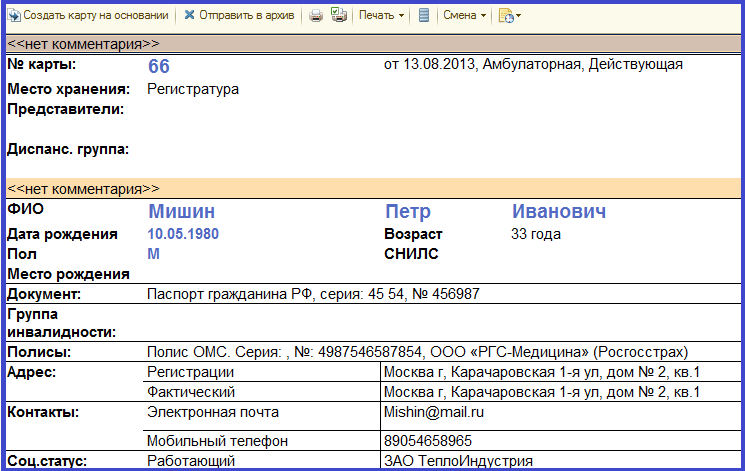
\includegraphics[width=\textwidth]{patientcard}
        \caption{Пример карты пациента}
        \label{fig:pc}
\end{figure}
\par
\begin{figure}[h!]
        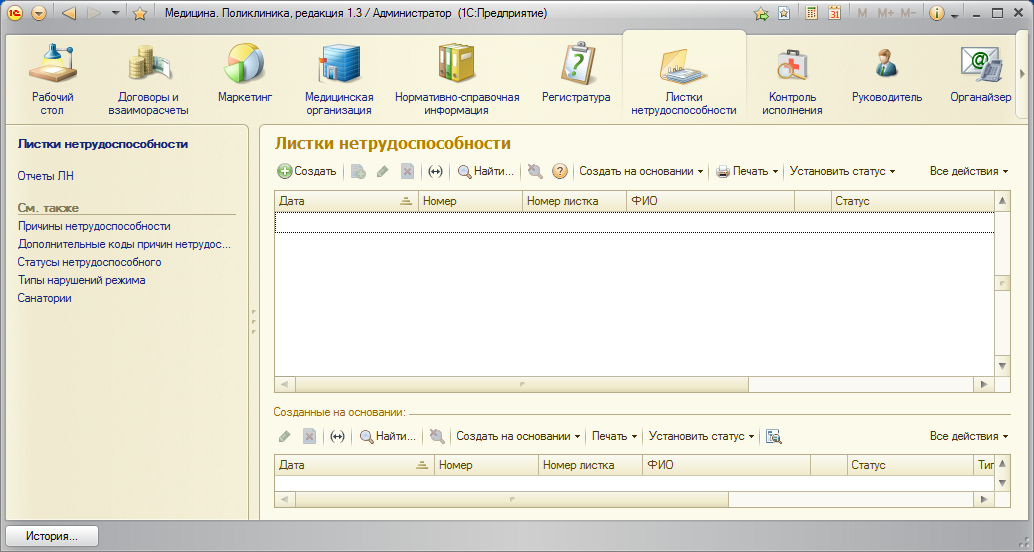
\includegraphics[width=\textwidth]{1cinterface}
        \caption{Пользовательский интерфейс «1С:Медицина. Поликлиника»}
        \label{fig:1c}
\end{figure}

Предварительную запись пациентов может осуществлять как регистратура, так и врачи при выполнении
назначений повторных приемов, консультаций, исследований, манипуляций. Для осуществления
оперативного планирования врачебному медицинскому персоналу и кабинетам задаются графики работы,
нормы загрузки, перечень выполняемых услуг. Оперативное планирование деятельности кабинетов
осуществляется по данным предварительной записи пациентов.\cite{1cclinic}
Можно выделить основные функциональные возможности «1С:Медицина. Поликлиника»:
\begin{enumerate}[noitemsep]
    \item Регистратура
    \item Листки нетрудоспособности (больничные)
    \item Договорной отдел
    \item Контроль исполнения медицинских услуг персоналом
    \item Руководитель и аналитическая (статистическая) служба
    \item Электронные медицинские карты
    \item Профосмотры
    \item Интернет запись на прием и обмен данными с сайтами
\end{enumerate}

\subsection{Сайт частных поликлиник «СМ-Клиника»}
Многопрофильный медицинский холдинг «СМ-Клиника»  - это сеть многопрофильных
медицинских центров для взрослых и детей, основанной в 2002 году. Услуги поликлиник предоставляются
на коммерческой основе.
Сайт компании доступен по адресу «http://www.smclinic.ru/».
Скриншот главной страницы сайта приведён на рис. \ref{fig:cc}.
На главной странице сайта можно выделить следующие функции:
\begin{itemize}[noitemsep]
    \item записаться на приём,
    \item личный кабинет, 
    \item услуги,
    \item анализы и диагностика.
\end{itemize}


\begin{figure}[t!]
        
\includegraphics[width=\textwidth]{cmclinic}
        \caption{Внешний вид сайта «СМ-Клиника»}
        \label{fig:cc}
\end{figure}

Функция «Записаться на приём» позволяет предварительно записаться на приём к лечащему врачу посредством заполнения
со стороны пользователя соответствующей формы (рис. \ref{fig:appdoc}).

\begin{figure}[t!]
        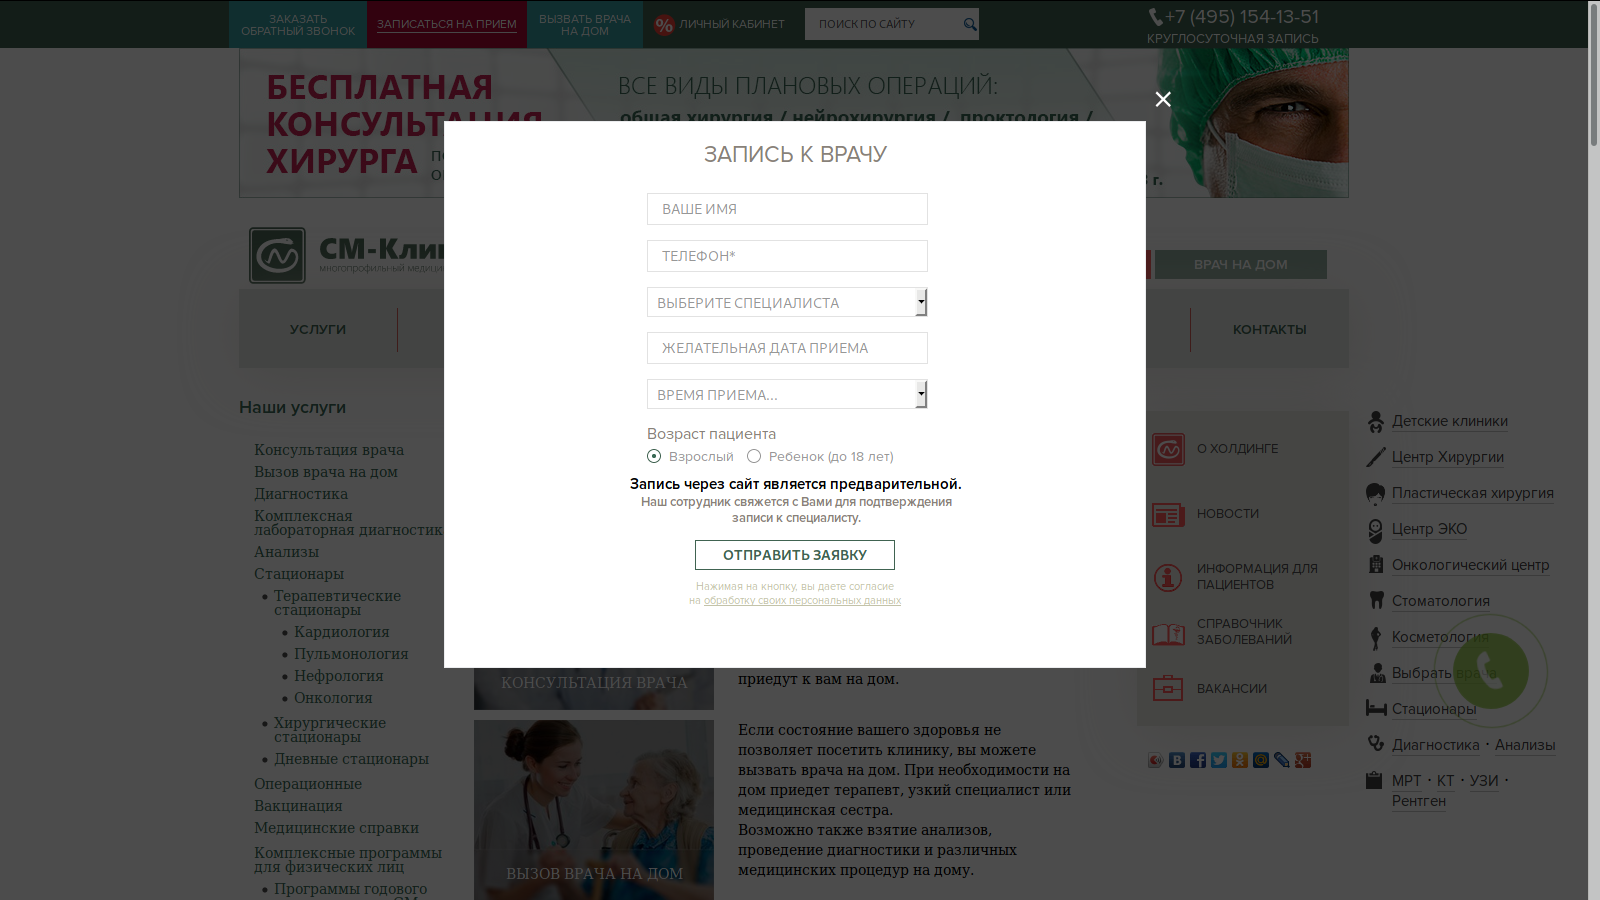
\includegraphics[width=\textwidth]{appdoc}
        \caption{Форма записи на приём к врачу в «СМ-Клиника»}
        \label{fig:appdoc}
\end{figure}
\cleardoublepage
\begin{figure}[t!]
        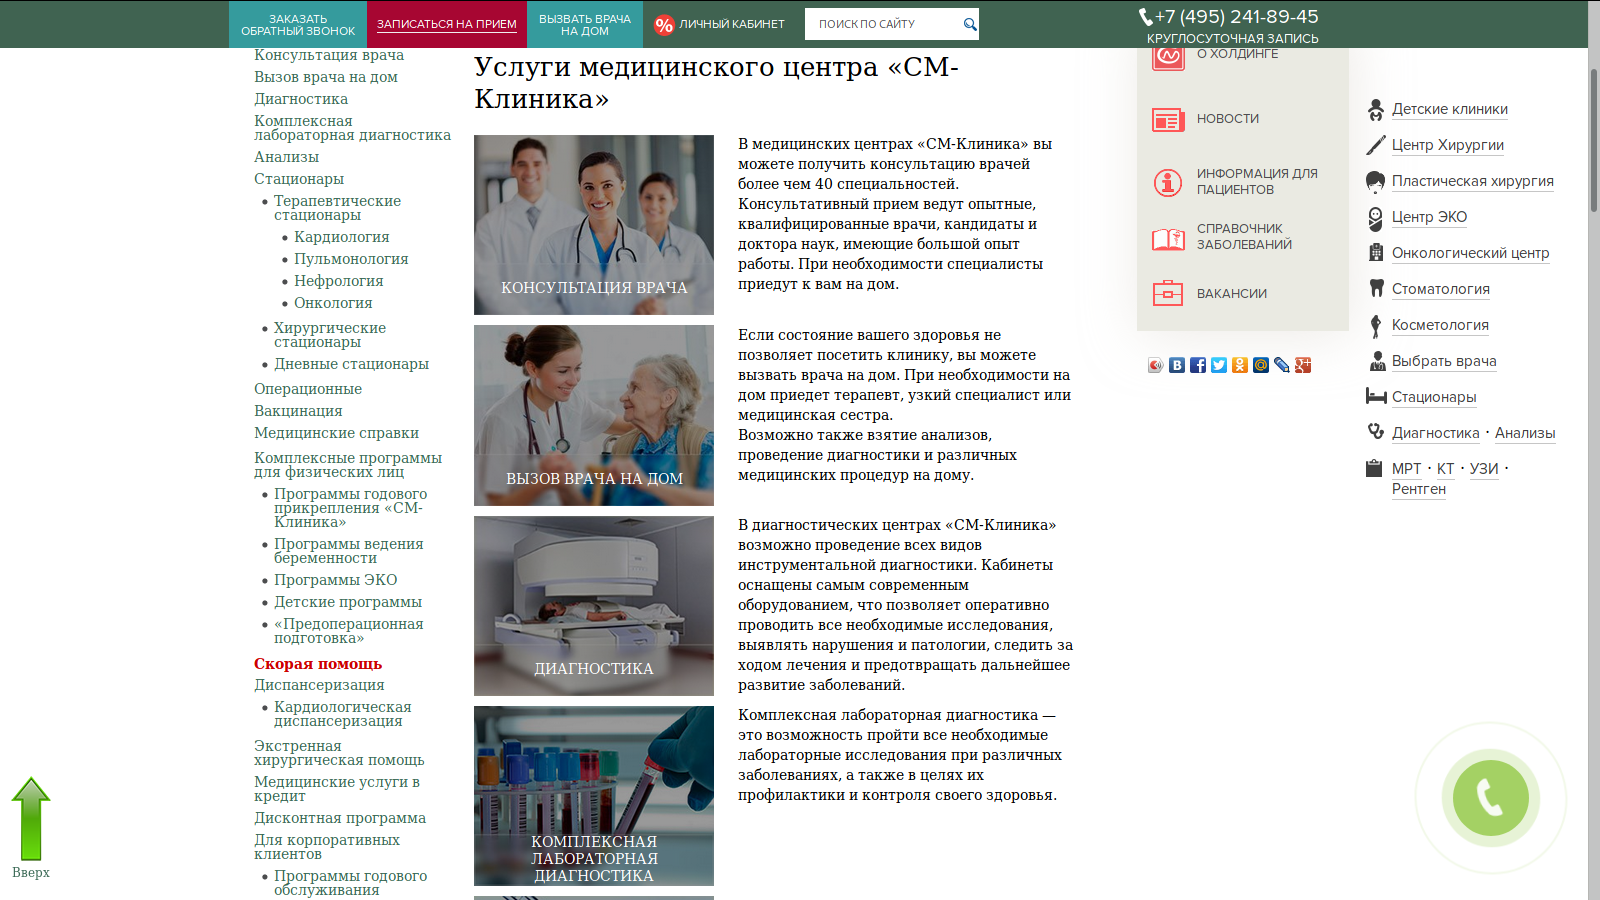
\includegraphics[width=\textwidth]{lkcm}
        \caption{Страница с перечнем предостваляемых услуг}
        \label{fig:lkcm}
\end{figure}

Функция «Личный кабинет» предоставляет широкий перечень возможностей для зарегистрированных
пользователей:

\begin{enumerate}[noitemsep]
    \item получить доступ к своей медицинской карте - увидеть детальную историю всех посещений
        клиники, фамилии лечащих докторов, их специализации, точные даты посещений и другую
        полезную информацию;

    \item посмотреть назначенную схему лечения, рекомендации лечащих врачей, назначенные
        обследования и др.;

    \item ознакомиться с результатами анализов и обследований, сохранить их на локальный компьютер или
        сразу распечатать;

    \item увидеть, когда лечащий врач пациента работает и какое время для приема на текущий момент у него
        свободно;

    \item самостоятельно записаться к врачу в удобное для пользователя время;

    \item посмотреть текущую скидку пользователя, актуальные акции и предложения клиник;

    \item оставить отзыв о враче или клинике.\cite{smclin}

\end{enumerate}
Функция «Услуги» позволяет подробно ознакомится c перечнем услуг предостваляемых поликлиникой
(рис. \ref{fig:lkcm}).


\subsection{Сравнение «1С:Медицина. Поликлиника» и сайта поликлиники «СМ-Клиника»}
Оба рассмотренных продукта, хотя и ориентированы на разные категории пользователей, имеют перечень
общих функций:
\begin{itemize}[noitemsep]
    \item доступ к электронной медицинской карте,
    \item запись на прием к врачу,
    \item ознакомиться с графиком лечащего врача,
    \item доступ к перечню предоставляемых поликлиникой услуг.
\end{itemize}

В рамках данной работы планируется создание единой платформы для
взамодейстивия пациентов с сотрудниками поликлиники. Проанализировав программные продукты решающие
схожие задачи в данной предметной области, можно выделить ряд функций которые необходимо
реализовать в процессе разработки:
\begin{enumerate}
            \item просмотр и/или редактирование медицинских карт,
            \item просмотр и/или редактирование результатов анализов,
            \item запись на приём к врачу,
            \item проcмотр и/или редактирование записей к врачам,
            \item создание листков нетрудоспособности,
            \item просмотр и/или редактирование результатов профосмотров,
            \item поиск всей информации касательно пациента,
            \item доступ к графику работы врачей,
            \item ознакомление с перечнем услуг, предоставляемых поликлиникой.
\end{enumerate}


\chapter{Концептуальное проектирование}
\section{Определение концептуального проектирования}
Концептуальное (инфологическое) проектирование — построение семантической модели предметной
области, то есть информационной модели наиболее высокого уровня абстракции. Такая модель создаётся
без ориентации на какую-либо конкретную СУБД и модель данных.
Чаще всего концептуальная модель базы данных включает в себя описание информационных объектов 
или понятий предметной области и связей между ними. Для визуализации концептуальной
модели часто используется диаграмма вариантов использования.\par
Диаграмма вариантов использования (ДВИ) — диаграмма, отражающая
отношения между действующими лицами и вариантами использования разрабатываемой системы, и
позволяющей описать систему на концептуальном уровне.
Основное назначение диаграммы — описание функциональности и поведения, позволяющее заказчику,
конечному пользователю и разработчику совместно обсуждать проектируемую или существующую
систему.\par

Действующее лицо - внешняя по отношению к ИС сущность, которая может
взаимодействовать с системой. Действующим лицом могут быть как люди, так и внешние системы или
устройства.\par
Вариант использования — возможность моделируемой системы (часть её функциональности), благодаря которой
пользователь может получить конкретный, измеримый и нужный ему результат. \cite{dbdesign}


\section{Концептуальная модель базы данных поликлиники}
В завершении анализа предметной области был выделен перечень функций которые необходимо реализовать
в рамках данной работы, и рассматривая данную ИС с точки зрения возможных вариантов использования, можно 
разделить эти функции между действующими лицами.\par
\noindent\textbf{Действующие лица:}
\begin{enumerate}[noitemsep]
    \item сотрудник регистратуры,
    \item врач,
    \item пациент.    
\end{enumerate}
Далее приведены варианты использования ИС каждым из действующих лиц. Сама же диаграмма показана на
рис. \ref{fig:ClinicDB}.
\begin{itemize}[noitemsep]
    \item Сотрудник регистратуры:
        \begin{enumerate}[noitemsep]
            \item поиск по медицинским картам пациентов,
            \item выдача информации по графику работы врачей,
            \item выдача информации информации о предоставляемых услугах,
            \item создание медицинской карты пациента,
            \item запись пациента к врачу.
        \end{enumerate}
    \item Врач:
        \begin{enumerate}[noitemsep]
            \item промотр истории болезней пациента.
            \item назначение лечения,
            \item назначение анализов,
            \item выписка рецептов пациентам,
            \item выписка листков нетрудоспособности.
        \end{enumerate}
    \item Пациент:
        \begin{enumerate}[noitemsep]
            \item ознакомление с графиком работы врачей,
            \item запись на приём к врачу,
            \item просмотр личной медицинской карты,
            \item получение информации о предоставляемых услугах.
        \end{enumerate}
\end{itemize}
\begin{figure}[h!]
        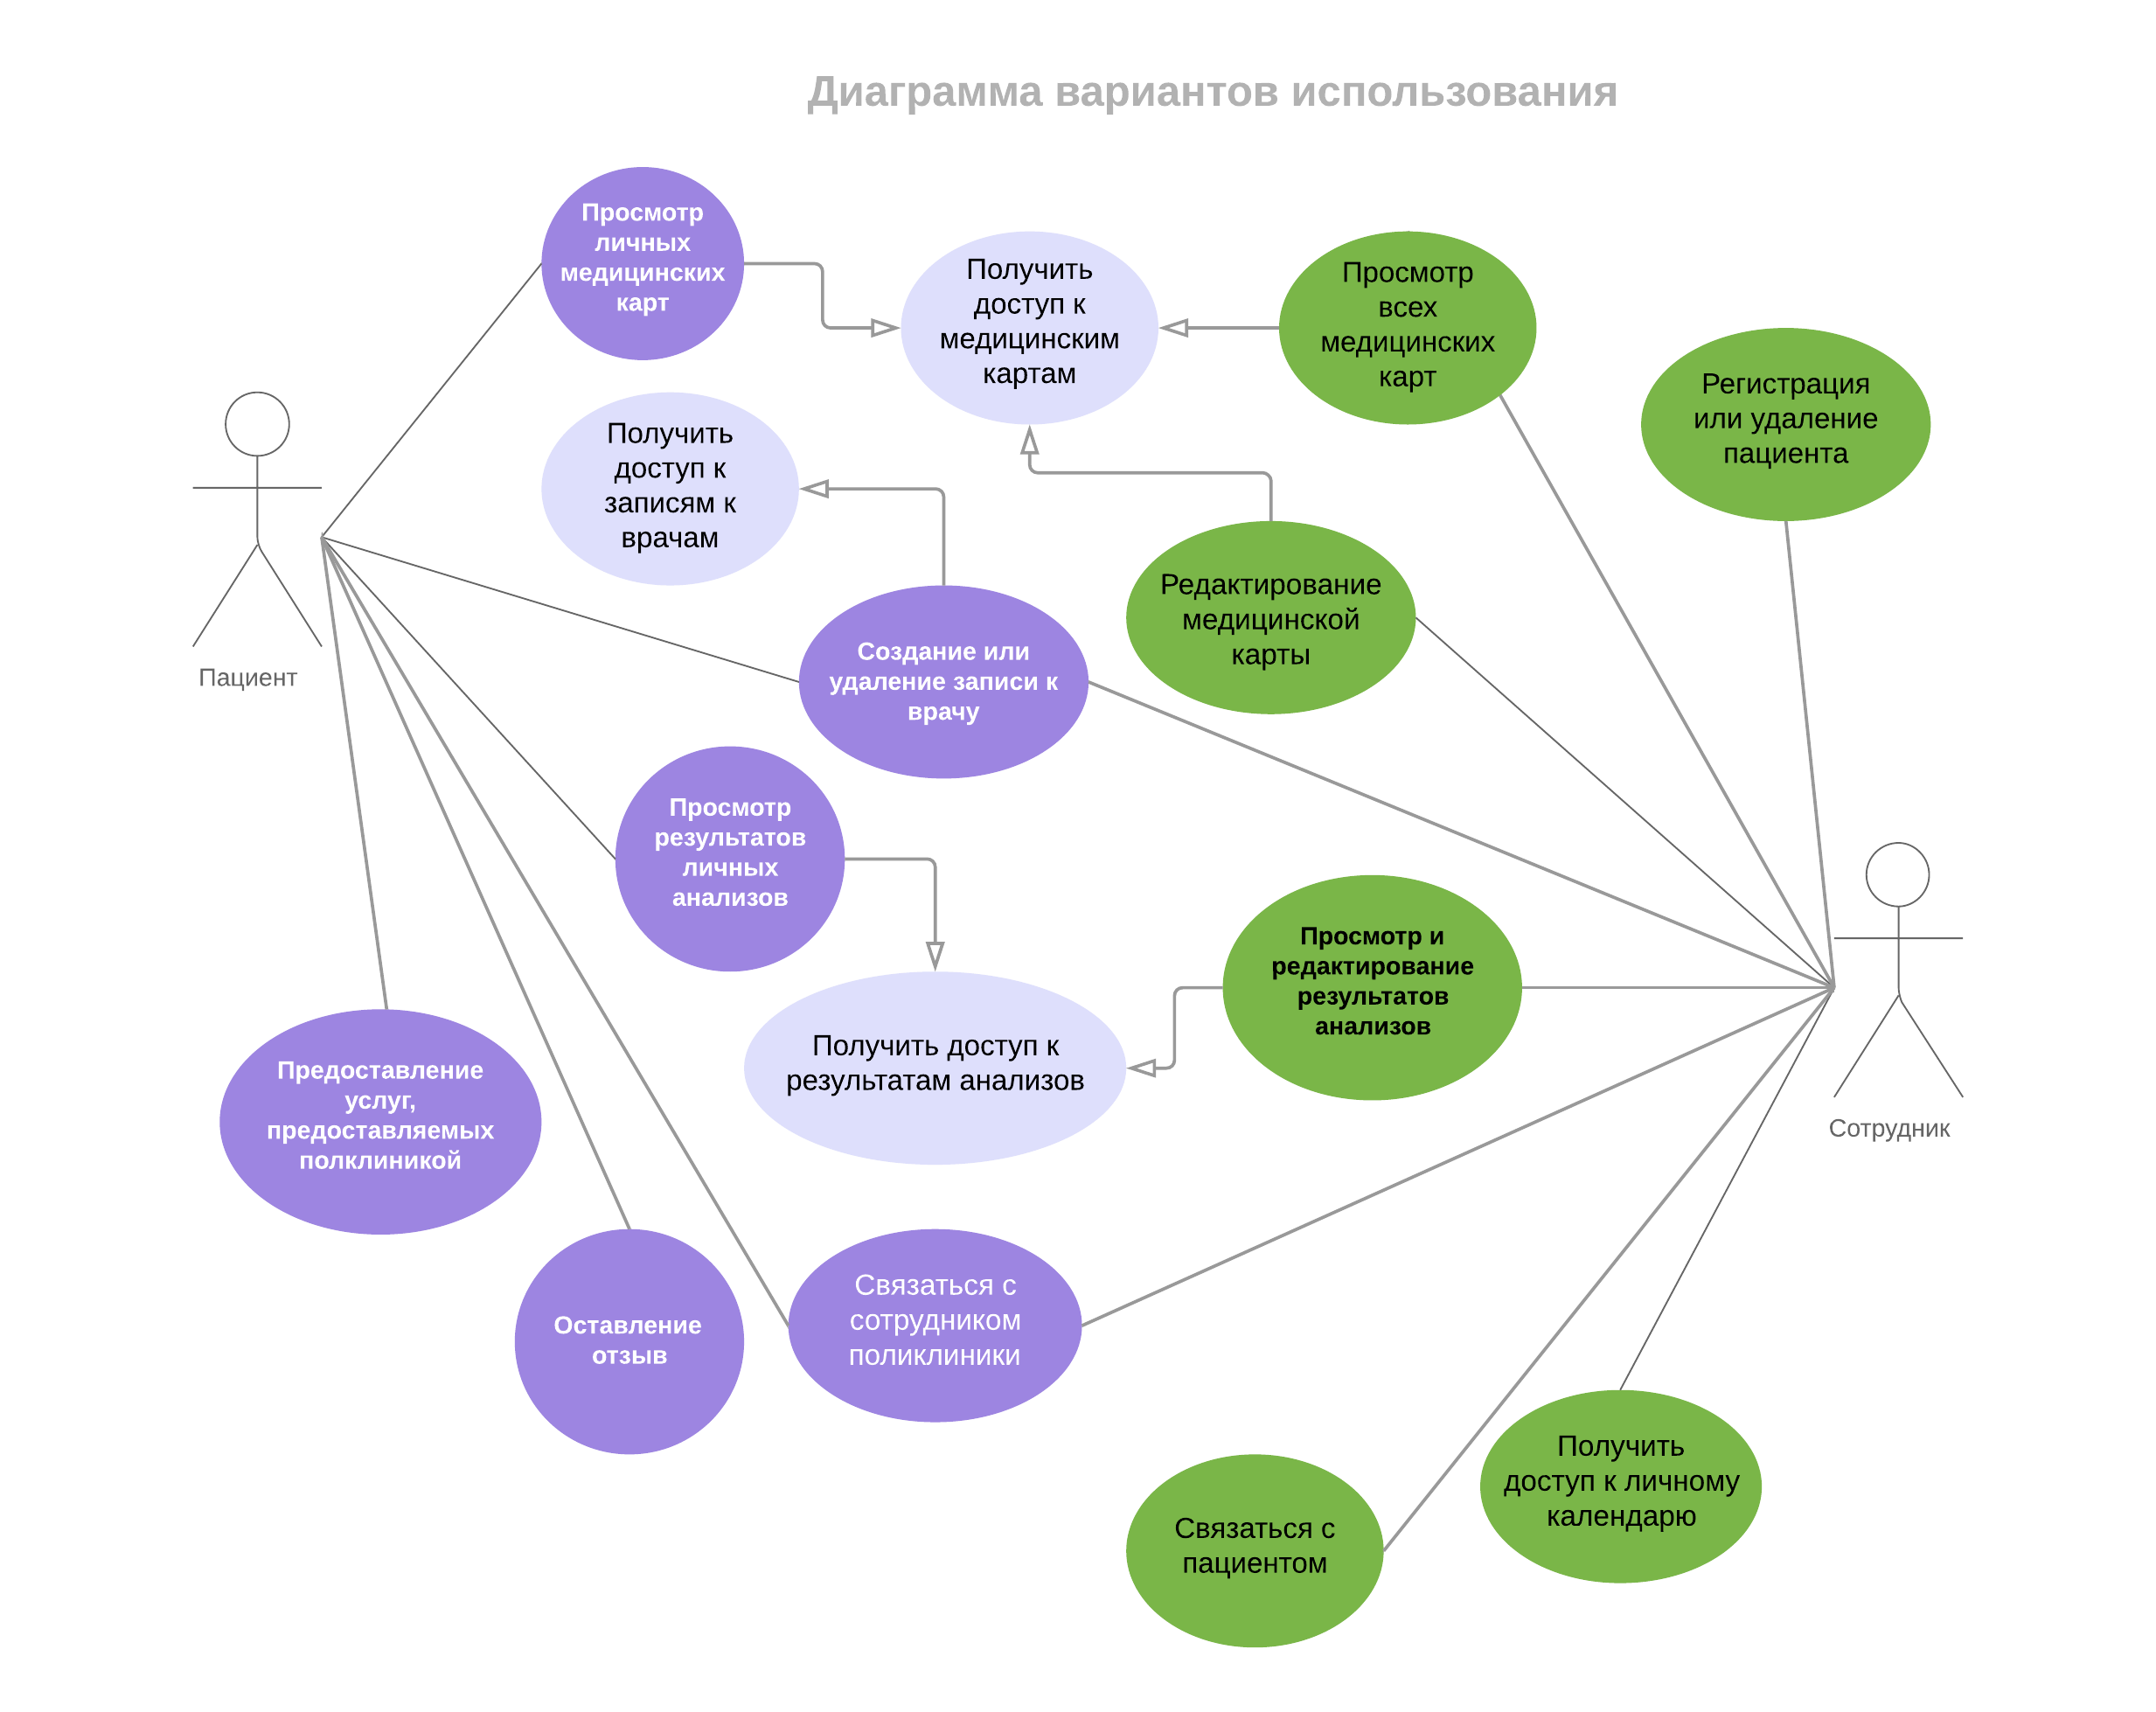
\includegraphics[width=\textwidth]{ClinicDB}
        \caption{Диаграмма вариантов использования}
        \label{fig:ClinicDB}
\end{figure}

Приняв во внимание всё вышесказанное, можно выделить данные, которые необходимо хранить в проектируемой базе данных.
\begin{enumerate}[noitemsep]
    \item информация о предоставляемых услугах,
    \item информация о пациентах,
    \item информация о сотрудниках поликлиники,
    \item информация о медицинских картах, т.е. их цифровые копии,
    \item информция графике приема пациентов врачами,
    \item информация о записях пациентов,
    \item информация об анализах,
    \item информация о выписанных рецептах,
    \item информация о выданных листках нетрудоспособности,
    \item информация о назначенных лечениях.
\end{enumerate}

Перечисленные данные можно подразделить на две группы:
\begin{itemize}[noitemsep]
    \item условно-постоянные(предоставляемые услуги, пациенты)
    \item оперативно-обновляемые(медицинские карты, график приема пациентов врачами, информация об
        анализах и т.д.).
\end{itemize}


\chapter{Логическое проектирование}
\section{Определение логического проектирования}
Логическое проектирование — создание схемы базы данных на основе конкретной модели
данных, например, реляционной модели данных. Для реляционной модели данных, логическая модель это
набор схем отношений, обычно с указанием первичных ключей, а также «связей» между
отношениями, представляющих собой внешние ключи.

Опираясь на концептуальную модель, проектируется логическую модель. Часто для выполнения этой
задачи используются различные модели данных, например ER-модель.
На этапе логического проектирования учитывается специфика конкретной модели данных, но может
не учитываться специфика конкретной СУБД. 

ER-модель (от англ. entity-relationship model, модель «сущность — связь») — модель данных,
позволяющая описывать концептуальные схемы предметной области.  ER-модель используется при
высокоуровневом (концептуальном) проектировании баз данных. С её помощью можно выделить ключевые
сущности и обозначить связи, которые могут устанавливаться между этими сущностями.\cite{dbdesign}


\vspace{0.7cm}
\section{ER-модель базы данных поликлиники}
На основе концептуальной модели поликлиники, описанной в конце предыдущей главы, можно
спроектировать ER-модель данной предметной области, и представить полученую модель с
помощью стандартной графической нотации ER-диаграммы (диаграммы сущность-связь).

\cleardoublepage
\begin{figure}[h!]
        
\includegraphics[width=\textwidth]{patappemp}
        \caption{Запись пациента к сотруднику (врачу)}
        \label{fig:patappemp}
\end{figure}

\noindent Тип связи ``Запись'' - M:N.\\
Класс принадлежности необязательный для обоих экземпляров сущностей.
Обоснование: Пациент может записаться к нулю или более сотрудникам (врачам), сотрудник может принять ноль или более
пациентов. 

\begin{figure}[h!]
        
\includegraphics[width=\textwidth]{medcvisemp}
        \caption{Посещения врача пациентом по медкарте}
        \label{fig:medcvisemp}
\end{figure}

\noindent Тип связи ``Посещения'' - M:N.\\
Класс принадлежности необязательный для обоих экземпляров сущностей.
Обоснование: Сотрудник может принимать нуль или более пациентов по медкарте, медкарта может
содержать информацию о нуль или более посещениях пациентам.

\begin{figure}[h!]
        
\includegraphics[width=\textwidth]{medcbelpat}
        \caption{Принадлежность медицинской карты пациенту}
        \label{fig:medcbelpat}
\end{figure}

\noindent Тип связи ``Владеет'' - 1:M.\\
Класс принадлежности обязательный для обоих экземпляров сущностей.\\
Обоснование: Пациент может владеть одной или более медкартами, медкарта должна принадлежать
только одному пациенту.

\begin{figure}[h!]
        
\includegraphics[width=\textwidth]{cardan}
        \caption{Назначение анализов пациенту по медкарте}
        \label{fig:cardan}
\end{figure}

\noindent Тип связи ``Анализ'' - M:N.\\
Класс принадлежности необязательный для обоих экземпляров сущностей.
Обоснование: Сотрудник может назначить анализ нуль или более пациентам по медкарте, по медкарте
анализ могут назначить нуль или более сотрудников.

\begin{figure}[h!]
        
\includegraphics[width=\textwidth]{empcuremedc}
        \caption{Назначение лечения пациенту по его медицинской карте}
        \label{fig:empcuremedc}
\end{figure}
\noindent Тип связи ``Лечение'' - M:N.\\
Класс принадлежности необязательный для обоих экземпляров сущностей.
Обоснование: Сотрудник может лечить нуль или более пациентов по медицинской карте, по
медицинской карте пациента могут лечить нуль или более сотрудников.
.

\begin{figure}[h!]
        
\includegraphics[width=\textwidth]{receipt}
        \caption{Выписывание врачом рецепта пациенту}
        \label{fig:receipt}
\end{figure}

\noindent Тип связи ``Рецепт'' - M:N.\\
Класс принадлежности необязательный для обоих экземпляров сущностей.\\
Обоснование: Сотрудник может выписать рецепты нуль или более пациентам,
пациент могут получить рецепты от нуль или более врачей.\par

\begin{figure}[h!]
        
\includegraphics[width=\textwidth]{servprovmedc}
        \caption{Оказание услуги пациенту по медкарте}
        \label{fig:servprovmedc}
\end{figure}

\noindent Тип связи ``Оказывается'' - M:N.\\
Класс принадлежности необязательный для обоих экземпляров сущностей.\\
Обоснование: Услуга может быть оказана нулю или более пациентам, пациент может получить нуль или
более услуг. 

\begin{figure}[h!]
        
\includegraphics[width=\textwidth]{empbolpat}
        \caption{Выписка больничного врачом пациенту}
        \label{fig:empbolpat}
\end{figure}

\noindent Тип связи ``Больничный'' - M:N.\\
Класс принадлежности необязательный для обоих экземпляров сущностей.\\
Обоснование: Сотрудник может выписать больничные нуль или более пациентам, пациент может получить
больничные от нуль или более сотрудников.

\begin{figure}[h!]
        
\includegraphics[width=\textwidth]{timetable}
        \caption{График работы сотрудников}
        \label{fig:timetable}
\end{figure}

\noindent Тип связи ``Принадлежит'' - 1:M.\\
Класс принадлежности обязательный для обоих экземпляров сущностей.
Обоснование: График работы может принадлежать только одному сотруднику, сотрудник может иметь
один или более графиков (например на каждый день недели).

\section{Преобразование ER-модели в реляционную}
\begin{enumerate}
    \item Связь ``Запись'' удовлетворяет условиям правила 6, откуда получаются следующие
        таблицы
        \begin{itemize}
            \item Пациент(\underline{Регистрационный номер}, ...);
            \item Сотрудник(\underline{Табельный номер}, ...);
            \item Запись(\underline{Табельный номер, Регистрационный номер}, ...).
        \end{itemize}
    \item Связь ``Посещения'' удовлетворяет условиям правила 6, откуда получаются следующие
        таблицы
        \begin{itemize}
            \item Пациент(\underline{Регистрационный номер}, ...);
            \item Сотрудник(\underline{Табельный номер}, ...);
            \item Посещения(\underline{Табельный номер, Регистрационный номер}, ...).
        \end{itemize}

    \item Связь ``Владеет'' удовлетворяет условиям правила 4, откуда получаются следующие таблицы
        \begin{itemize}
            \item Пациент(\underline{Регистрационный номер}, ...);
            \item Медкарта(\underline{Номер медкарты}, Регистрационный номер, ...).
        \end{itemize}
    \item Связь ``Анализ'' удовлетворяет условиям правила 6, откуда получаются следующие
        таблицы
        \begin{itemize}
            \item Сотрудник(\underline{Табельный номер}, ...);
            \item Медкарта(\underline{Номер медкарты}, ...).
            \item Анализ(\underline{Номер анализа}Табельный номер, номер медкарты, ...).
        \end{itemize}
    \item Связь ``Лечение'' удовлетворяет условиям правила 6, откуда получаются следующие таблицы
        \begin{itemize}
            \item Сотрудник(\underline{Табельный номер}, ...);
            \item Медкарта(\underline{Номер медкарты}, ...);
            \item Лечение(\underline{Табельный номер, номер медкарты, дата назначения}, ...).
        \end{itemize}
    \item Связь ``Рецепт'' удовлетворяет условиям правила 6, откуда получаются следующие таблицы
        \begin{itemize}
            \item Сотрудник(\underline{Табельный номер}, ...);
            \item Пациент(\underline{Регистрационный номер}, ...);
            \item Рецепт(\underline{Табельный номер, Регистрационный номер, дата выписки}, ...).
        \end{itemize}
    \item Связь ``Оказывается'' удовлетворяет условиям правила 6, откуда получаются следующие
        таблицы
        \begin{itemize}
            \item Услуга(\underline{Номер услуги}, ...).
            \item Медкарта(\underline{Номер медкарты}, ...);
            \item Оказание(\underline{Название,Номер медкарты, дата оказания} ...);
        \end{itemize}
    \item Связь ``Больничный'' удовлетворяет условиям правила 6, откуда получаются следующие
        таблицы
        \begin{itemize}
            \item Пациент(\underline{Регистрационный номер}, ...);
            \item Сотрудник(\underline{Табельный номер}, ...);
            \item Больничный(\underline{Табельный номер, Регистрационный номер, дата выдачи}, ...);
        \end{itemize}
    \item Связь ``Принадлежит'' удовлетворяет условиям правила 4, откуда получаются следующие
        таблицы
        \begin{itemize}
            \item Сотрудник(\underline{Табельный номер}, ...);
            \item График(\underline{День недели, Табельный номер}, ...);
        \end{itemize}
\end{enumerate}
В итоге получается 12 таблиц, которые приведены ниже с перечнем всех относящихся к ним атрибутам.
\begin{enumerate}
            \item Пациент(\underline{Регистрационный номер}, ФИО, дата рождения, пол, адрес
                проживания, контактный телефон, пароль от ЛК);
            \item Сотрудник(\underline{Табельный номер}, ФИО, должность, стаж, дата рождения, пол, адрес
                проживания, контактный телефон, пароль от ЛК);
            \item Запись(\underline{Табельный номер, Регистрационный номер}, дата и время записи).
            \item Посещения(\underline{Табельный номер, Регистрационный номер, дата посещения},
                цель визита).
            \item Медкарта(\underline{Номер медкарты}, Регистрационный номер, дата заведения, тип).
            \item Анализ(\underline{Табельный номер, номер медкарты}, дата сдачи, вид анализа,
                результат).
            \item Лечение(\underline{Табельный номер, номер медкарты, дата назначения},
                заболевание, назначенное лечение).
            \item Услуга(\underline{Название}, описание, стоимость).
            \item Оказание(\underline{Название,Номер медкарты, дата оказания}, комментарий).
            \item Рецепт(\underline{Табельный номер, Регистрационный номер, дата выписки}, медикаменты).
            \item Больничный(\underline{Табельный номер, Регистрационный номер, дата выдачи},
                начало больничного,окончание больничного, место работы/обучения);
            \item График(\underline{День недели, Табельный номер}, начало смены, конец смены,
                перерыв);
\end{enumerate}



\chapter{Физическое проектирование}
Физическое проектирование — создание схемы базы данных для конкретной СУБД. Специфика конкретной
СУБД может включать в себя ограничения на именование объектов базы данных, ограничения на
поддерживаемые типы данных и т. п. Кроме того, специфика конкретной СУБД при физическом
проектировании включает выбор решений, связанных с физической средой хранения данных (выбор методов
управления дисковой памятью, разделение БД по файлам и устройствам, методов доступа к данным),
создание индексов и т. д.\cite{dbdesign} 


\section{Выбор СУБД}
В данной работе для реализации базы данных поликлиники была выбрана реляционная СУБД
SQLite. Такой выбор обоснован спецификой предметной области, а именно относительно небольшим
объёмом хранимых данных и средней частотой обращения к базе данных. SQLite является
встраиваемой, т.е. вместо использования привычной парадигмы клиент-сервер, SQLite представляет из
себя библиотеку с интерфейсами для многих языков программирования. Этот факт делает SQLite
чрезвычайно компактным и быстрым, т.к. СУБД встраиваится напрямую в разрабатываемое приложение.
Несмотря на свою простоту данная СУБД может обслуживать базы данных размером до 140 террабайт и
поддерживает параллельный доступ к БД несколькими процессами. Помимо этого SQLite выполняет
поддавляющее большинство требований изложенных в стандарте SQL, а также соблюдает ACID-требования
(Atomicity, Consistency, Isolation, Durability).\cite{sqlite}


\section{Схема БД поликлиники}
На основании ER-модели, полученной в конце предыдущей главы, где были описаны таблицы и их атрибуты,
далее приведены окончательные структуры таблиц, какими они будут в СУБД SQLite. Поля перечислены в
том же порядке, который был описан ранее. SQL операторы
использованные для создания таблиц приведены в приложении А, в приложении Б приведены примеры их
заполнения.


\begin{table}[h]
    \caption{ } 
    \begin{subtable}[t]{\textwidth}
        \caption{\textbf{«Пациент»}}
    \begin{tabularx}{\textwidth}{| X | X | X | c | c | c | X |}
        \hline
        \textbf{Столбец} & \textbf{Тип данных} & \textbf{Нуль?} & \textbf{Ключ} & \textbf{По
        умолч.} & \textbf{Огранич.} & \textbf{Ссылка} \\ \hline
        regid & integer & not null & первичный & & & \\ \hline
        fio & text & not null & & & & \\ \hline
        birthdate & date & not null & & & < date('now') & \\ \hline
        gender & char(1) & not null & & & `М' или `Ж' & \\ \hline
        address & text & & & & & \\ \hline
        pnumber & text & & & & & \\ \hline
        password & text & not null & & abs(random()) & & \\ \hline
    \end{tabularx}
    \end{subtable}
    \label{table:pat}
\end{table}

\begin{table}[h]
    \caption{ } 
    \begin{subtable}[t]{\textwidth}
        \caption{\textbf{«Медкарта»}}
    \begin{tabularx}{\textwidth}{| X | X | c | c | c | c | X |}
        \hline
        \textbf{Столбец} & \textbf{Тип данных} & \textbf{Нуль?} & \textbf{Ключ} & \textbf{По
        умолч.} & \textbf{Огранич.} & \textbf{Ссылка} \\ \hline
        cardid & integer & not null & первичный & & & \\ \hline
        regid & integer & not null & внешний & & & Пациент (regid) \\ \hline
        crdate & date & not null & & date('now') & & \\ \hline
        type & text & & & & & \\ \hline
    \end{tabularx}
    \end{subtable}
    \label{table:medcard}
\end{table}

\begin{table}[h]
    \caption{ } 
    \begin{subtable}[t]{\textwidth}
        \caption{\textbf{«Сотрудник»}}
    \begin{tabularx}{\textwidth}{| X | X | X | c | c | c | X |}
        \hline
        \textbf{Столбец} & \textbf{Тип данных} & \textbf{Нуль?} & \textbf{Ключ} & \textbf{По
        умолч.} & \textbf{Огранич.} & \textbf{Ссылка} \\ \hline
        tabid & integer & not null & первичный & & &  \\ \hline
        fio & text & not null & & & & \\ \hline
        position & text & not null & & & & \\ \hline
        experien & integer & not null & & 0 & < 100 & \\ \hline
        birthdate & date & not null & & & < date('now') & \\ \hline
        gender & char(1) & not null & & & `М' или `Ж' & \\ \hline
        address & text & & & & & \\ \hline
        pnumber & text & & & & & \\ \hline
        password & text & not null & & abs(random()) & & \\ \hline
    \end{tabularx}
    \end{subtable}
    \label{table:emp}
\end{table}

\begin{table}[h]
    \caption{ } 
    \begin{subtable}[t]{\textwidth}
        \caption{\textbf{«Анализ»}}
    \begin{tabularx}{\textwidth}{| X | X | c | c | c | c | X |}
        \hline
        \textbf{Столбец} & \textbf{Тип данных} & \textbf{Нуль?} & \textbf{Ключ} & \textbf{По
        умолч.} & \textbf{Огранич.} & \textbf{Ссылка} \\ \hline
        anid & integer & not null & первичный & & & \\ \hline
        tabid & integer & not null & внешний & & & Сотрудник (tabid) \\ \hline
        cardid & integer & not null & внешний & & & Медкарта (cardid) \\ \hline
        passdate & date & not null & & date('now') & & \\ \hline
        type & text & not null & & & & \\ \hline
        result & text & & & & & \\ \hline
    \end{tabularx}
    \end{subtable}
    \label{table:analysis}
\end{table}

\begin{table}[h]
    \caption{ } 
    \begin{subtable}[t]{\textwidth}
        \caption{\textbf{«Запись»}}
    \begin{tabularx}{\textwidth}{| X | X | X | X | X | X | X |}
        \hline
        \textbf{Столбец} & \textbf{Тип данных} & \textbf{Нуль?} & \textbf{Ключ} & \textbf{По
        умолч.} & \textbf{Огранич.} & \textbf{Ссылка} \\ \hline
        tabid & integer & not null & первичный, внешний & & & Сотрудник (tabid) \\ \hline
        regid & integer & not null & первичный, внешний & & & Пациент (regid)  \\ \hline
        recdatetime & datetime & not null & & & & \\ \hline
    \end{tabularx}
    \end{subtable}
    \label{table:rec}
\end{table}



\begin{table}[h]
    \caption{ }
    \begin{subtable}[t]{\textwidth}
        \caption{\textbf{«Посещения»}}
    \begin{tabularx}{\textwidth}{| X | X | c | X | c | c | X |}
        \hline
        \textbf{Столбец} & \textbf{Тип данных} & \textbf{Нуль?} & \textbf{Ключ} & \textbf{По умолч.} & \textbf{Огранич.} & \textbf{Ссылка} \\ \hline
            tabid & integer & not null & первичный, внешний & & & Сотрудник (tabid) \\ \hline

            regid & integer & not null & первичный, внешний & & & Пациент (regid)\\ \hline
            visdate & date & not null & первичный & date('now') & & \\ \hline
            visgoal & text & not not & & & & \\ \hline
    \end{tabularx}
    \end{subtable}
    \label{table:visit}
\end{table}

\begin{table}[h]
    \caption{ } 
    \begin{subtable}[t]{\textwidth}
        \caption{\textbf{«Рецепт»}}
    \begin{tabularx}{\textwidth}{| X | X | c | X | c | c | X |}
        \hline
        \textbf{Столбец} & \textbf{Тип данных} & \textbf{Нуль?} & \textbf{Ключ} & \textbf{По
        умолч.} & \textbf{Огранич.} & \textbf{Ссылка} \\ \hline
            tabid & integer & not null & первичный, внешний & & & Сотрудник (tabid) \\ \hline

            regid & integer & not null & первичный, внешний & & & Пациент (regid)\\ \hline
            issuedate & date & not null & первичный & date('now') & & \\ \hline
        medicine & text & not null & & & & \\ \hline
    \end{tabularx}
    \end{subtable}
    \label{table:receipt}
\end{table}

\begin{table}[h]
    \caption{ } 
    \begin{subtable}[t]{\textwidth}
        \caption{\textbf{«Услуга»}}
    \begin{tabularx}{\textwidth}{| X | X | c | X | c | c | X |}
        \hline
        \textbf{Столбец} & \textbf{Тип данных} & \textbf{Нуль?} & \textbf{Ключ} & \textbf{По
        умолч.} & \textbf{Огранич.} & \textbf{Ссылка} \\ \hline
        name & integer & not null & первичный & & & \\ \hline
        descrip & text & not null & & & & \\ \hline
        cost & integer & not null & & 0 & & \\ \hline
    \end{tabularx}
    \end{subtable}
    \label{table:serv}
\end{table}


\begin{table}[h]
    \caption{ } 
    \begin{subtable}[t]{\textwidth}
        \caption{\textbf{«Оказание»}}
    \begin{tabularx}{\textwidth}{| X | X | c | X | c | c | X |}
        \hline
        \textbf{Столбец} & \textbf{Тип данных} & \textbf{Нуль?} & \textbf{Ключ} & \textbf{По
        умолч.} & \textbf{Огранич.} & \textbf{Ссылка} \\ \hline
        name & text & not null & первичный, внешний & & &  Услуга (name) \\ \hline
        regid & integer & not null & первичный, внешний & & & Пациент (regid) \\ \hline
        provdate & date & not null & первичный & datetime('now') &  & \\ \hline
        comment & text & & & & & \\ \hline
    \end{tabularx}
    \end{subtable}
    \label{table:servprovision}
\end{table}


\begin{table}[h]
    \caption{ } 
    \begin{subtable}[t]{\textwidth}
        \caption{\textbf{«Лечение»}}
    \begin{tabularx}{\textwidth}{| X | X | c | X | c | c | X |}
        \hline
        \textbf{Столбец} & \textbf{Тип данных} & \textbf{Нуль?} & \textbf{Ключ} & \textbf{По
        умолч.} & \textbf{Огранич.} & \textbf{Ссылка} \\ \hline
        tabid & integer & not null & первичный, внешний & & & Сотрудник (tabid) \\ \hline
        cardid & integer & not null & первичный, внешний & & & Медкарта (cardid) \\ \hline
        trdate & date & not null & первичный & date('now') & & \\ \hline 
        illness & text & & & & & \\ \hline
        treatment & text & & & & & \\ \hline
    \end{tabularx}
    \end{subtable}
    \label{table:treat}
\end{table}

\cleardoublepage
\begin{table}[t!]
    \caption{ } 
    \begin{subtable}[t]{\textwidth}
        \caption{\textbf{«Больничный»}}
    \begin{tabularx}{\textwidth}{| X | X | c | X | c | X | X |}
        \hline
        \textbf{Столбец} & \textbf{Тип данных} & \textbf{Нуль?} & \textbf{Ключ} & \textbf{По
        умолч.} & \textbf{Огранич.} & \textbf{Ссылка} \\ \hline
            tabid & integer & not null & первичный, внешний & & & Сотрудник (tabid) \\ \hline

            regid & integer & not null & первичный, внешний & & & Пациент (regid)\\ \hline
            issuedate & date & not null & первичный & date('now') & & \\ \hline
        stdate & date & not null & & & & \\ \hline
        endate & date & not null & & & endate > stdate & \\ \hline
        destn & text & not null & & & & \\ \hline
    \end{tabularx}
    \end{subtable}
    \label{table:sickleave}
\end{table}

\begin{table}[h]
    \caption{ } 
    \begin{subtable}[t]{\textwidth}
        \caption{\textbf{«График»}}
    \begin{tabularx}{\textwidth}{| X | X | X | X | X | X | X |}
        \hline
        \textbf{Столбец} & \textbf{Тип данных} & \textbf{Нуль?} & \textbf{Ключ} & \textbf{По
        умолч.} & \textbf{Огранич.} & \textbf{Ссылка} \\ \hline
        tabid & integer & not null & первичный, внешний & & & Сотрудник (tabid) \\ \hline
        weekday & text & not null & первичный & & & \\ \hline
        shiftst & integer & not null & & & & \\ \hline
        shiftend & integer & not null & & & & \\ \hline
        break & integer & not null & & & & \\ \hline
    \end{tabularx}
    \end{subtable}
    \label{table:timetable}
\end{table}

Таблица «Пациент» содержит персональные данные пациентов поликлиники (см. табл.
\ref{table:pat})\par
Таблица «Медкарта» содержит информацию о медкартах пациентов, дополнительные ограничения на таблицу
это требования уникальности регистрационного номера пациента и типа медкарты unique(regid, type) (см. табл.
\ref{table:medcard}).\par
Таблица «Сотрудник» содержит информацию о сотрудниках поликлиники (см. табл. \ref{table:emp}).\par
Таблица «Анализ» содержит информацию об анализах назначенных врачамм пациентам поликлиники (см.
табл. \ref{table:analysis}).\par
Таблица «Запись» содержит информацию о записях пациентов к врачам поликлиники,
дополнительные ограничения на таблицу это требования уникальности табельного номера врача и времени
записи unique(tabid, recdatetime), а также уникальность регистрационного номера пациента и времени
записи unique(regid, recdatetime) (см. табл. \ref{table:rec}).\par
Таблица «Посещения» содержит информацию о факте посещения врача пациентом (см. табл.
\ref{table:visit}).\par
Таблица «Рецепт» содержит информацию о рецептах выписанных врачами пациентам (см. табл.
\ref{table:receipt}).\par
Таблица «Услуга» содержит информацию об услугах оказываемых поликлиникой (см. табл. \ref{table:serv}).\par
Таблица «Оказание» содержит информацию о факте оказания услуги пациенту (см. табл.
\ref{table:servprovision}).\par
Таблица «Лечение» содержит информацию о лечениях назначаемых врачами пациентам (см. табл.
\ref{table:treat}).\par
Таблица «Больничный» содержит информацию о листках нетрудоспособности выданных врачами пациентам
(см. табл. \ref{table:sickleave}).\par
Таблица «График» содержит информацию о графиках сотрудников.
(см. табл. \ref{table:timetable}).\par




На рис. \ref{fig:clinic} можно ознакомиться с общей схемой БД. Визуализаация была
произведена средствами программного продукта DataGrip версия 2017.2.
\begin{figure}[h!]
        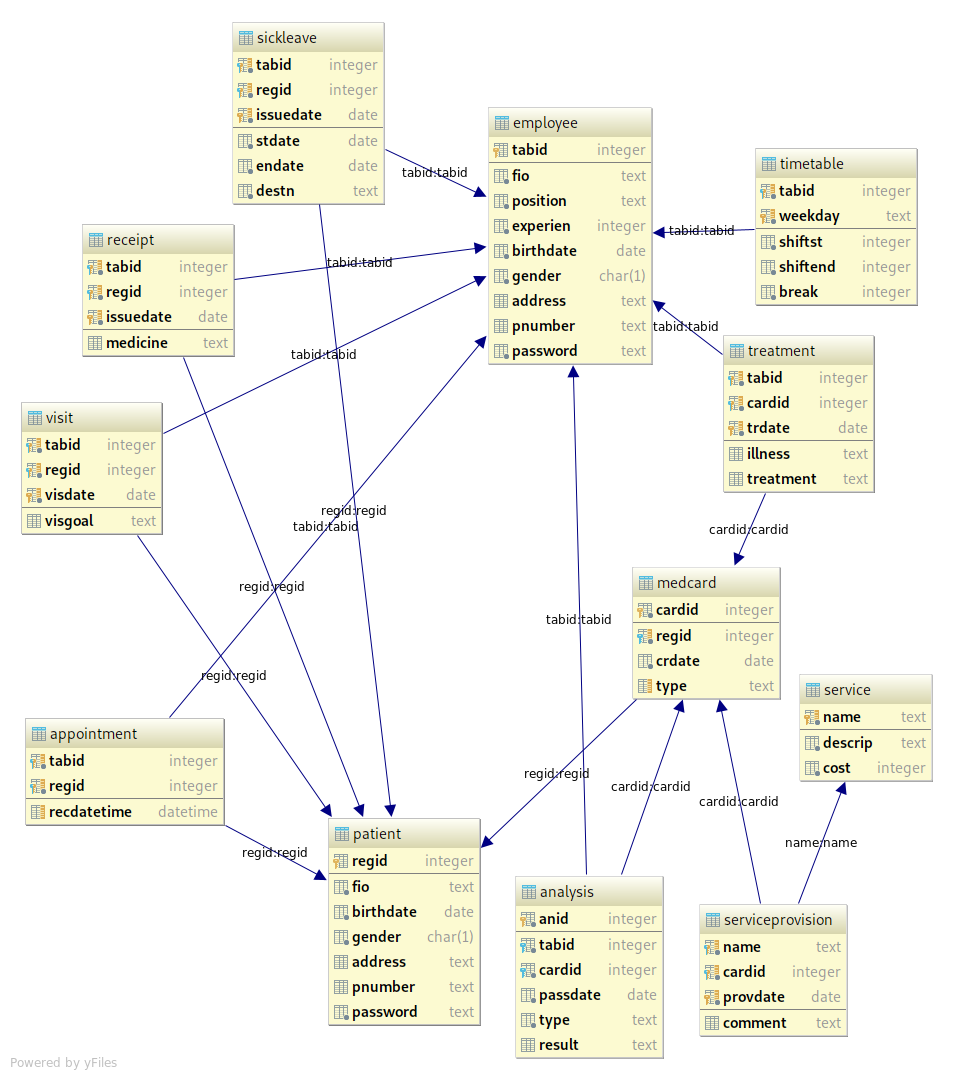
\includegraphics[scale=0.52]{clinic}
        \caption{Схема базы данных поликлиники}
        \label{fig:clinic}
\end{figure}


\chapter*{Заключение}
\addcontentsline{toc}{chapter}{Заключение}
Целью данной работы является проектирование базы данных для поликлиники. 
В связи с ростом человеческого населения, и высокой степени бюрократизации поликлиник, проблема
автоматизации работы подобного рода учреждений особенно актуальна, так как это непосредственно
сказывается на качестве оказываемых услуг. В ходе выполнения работы были достигнуты следующие цели: 

\begin{enumerate}[noitemsep]
        \vspace{-5pt}
    \item Была проанализирована предметная область поликлиника и её особенности, также были
        приведены аргументы в пользу необходимости в автоматизации. Были рассмотрены две существующих
        продукта, которые в той или иной мере решают проблему автоматизации, предоставляемые ими
        функции и их специфика. На основании анализа предметной области был выделен перечень
        функций для будущей реализации.
    \item Следующим этапом стало концептуальное проектирование, в ходе которого были выделены
        два 
        действующих лица (сотрудник, пациент), для которыx была составлена
        диаграмма вариантов использования.
    \item Далее в ходе логического проектирования была создана ER-модель базы данных, где были
        определены основные сущности и их взаимодействия. Для визуализации ER-модели были
        использованы ER-диаграммы. В завершении данного этапа были построена схема БД в виде набора
        схем отношений.
    \item Завершающим этапом стало физическое проектирование, в ходе которого в СУБД SQLite была
        создана база данных поликлиники со всеми таблицами, определенных на предыдущем этапе, после
        чего все таблицы были заполнены данными.
\end{enumerate}
    В дальнейшем планируется создание программного продукта, который предоставляет
        пользователю интерфейс для работы с созданной в данной работе базой данных.

\addcontentsline{toc}{chapter}{Литература}
\bibliography{b}{}

\newpage
\hfill\textbf{Приложение А}
\addcontentsline{toc}{chapter}{Приложение А}
\setcounter{lstlisting}{0}


\lstinputlisting[title=1. Создание таблицы «Пациент», label=list:cpat, style=csql]{code/cpatient.sql}
\lstinputlisting[title=2. Создание таблицы «Сотрудник», label=list:cemp, style=csql]{code/cemployee.sql}
\lstinputlisting[title=3. Создание таблицы «Запись», label=list:rec, style=csql]{code/cappointment.sql}
\newpage
\lstinputlisting[title=4. Создание таблицы «Медкарта», label=list:medc, style=csql]{code/cmedcard.sql}
\lstinputlisting[title=5. Создание таблицы «Посещения», label=list:medc, style=csql]{code/cvisit.sql}
\lstinputlisting[title=6. Создание таблицы «Анализ», label=list:res,
style=csql]{code/canalysis.sql}
\lstinputlisting[title=7. Создание таблицы «Услуга», label=list:patlink,
style=csql]{code/cservice.sql}
\newpage
\lstinputlisting[title=8. Создание таблицы «Оказание», label=list:emplink,
style=csql]{code/cserviceprovision.sql}
\lstinputlisting[title=9. Создание таблицы «Лечение», label=list:treat, style=csql]{code/ctreatment.sql}
\lstinputlisting[title=10. Создание таблицы «Рецепт», label=list:serv, style=csql]{code/creceipt.sql}
\lstinputlisting[title=11. Создание таблицы «Больничный», label=list:reserv,
style=csql]{code/csickleave.sql}
\lstinputlisting[title=12. Создание таблицы «График», label=list:timetable,
style=csql]{code/ctimetable.sql}


\newpage
\hfill\textbf{Приложение Б}
\setcounter{figure}{0}
\counterwithout{figure}{chapter}
\addcontentsline{toc}{chapter}{Приложение Б}

\subsection*{Заполнение таблиц данными}
\setlength{\textfloatsep}{2pt}
\begin{figure}[h!]
        \center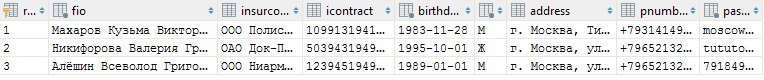
\includegraphics[scale=1]{patient}
        \caption{Заполнение таблицы «Пациент»}
        \label{fig:patient}
\end{figure}

\vspace{0.00mm}

\begin{figure}[h!]
        \center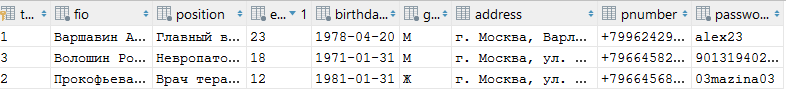
\includegraphics[scale=0.83]{employee}
        \caption{Заполнение таблицы «Сотрудник»}
        \label{fig:employee}
\end{figure}

\vspace{0.00mm}

\begin{figure}[h!]
        \center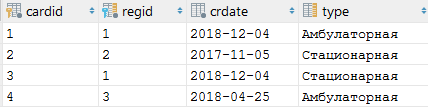
\includegraphics[scale=1]{medcard}
        \caption{Заполнение таблицы «Медкарта»}
        \label{fig:medcard}
\end{figure}

\vspace{0.00mm}

\begin{figure}[h!]
        \center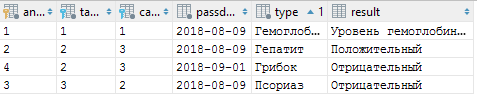
\includegraphics[scale=1]{analysis}
        \caption{Заполнение таблицы «Анализ»}
        \label{fig:employee}
\end{figure}

\vspace{0.00mm}

\begin{figure}[h!]
        \center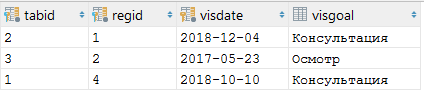
\includegraphics[scale=1]{visit}
        \caption{Заполнение таблицы «Посещения»}
        \label{fig:visit}
\end{figure}

\vspace{0.00mm}

\begin{figure}[h]
        \center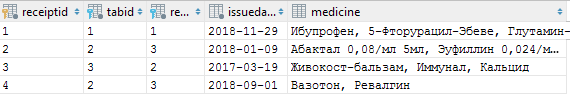
\includegraphics[scale=1]{ireceipt}
        \caption{Заполнение таблицы «Рецепт»}
        \label{fig:ireceipt}
\end{figure}

\vspace{0.00mm}

\begin{figure}[h]
        \center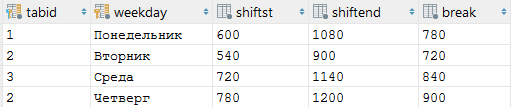
\includegraphics[scale=1]{itimetable}
        \caption{Заполнение таблицы «График»}
        \label{fig:itimetable}
\end{figure}

\vspace{0.00mm}

\begin{figure}[h]
        \center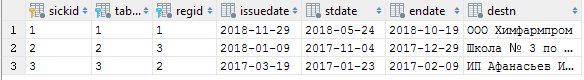
\includegraphics[scale=1]{sickleave}
        \caption{Заполнение таблицы «Больничный»}
        \label{fig:sickleave}
\end{figure}

\vspace{0.00mm}

\begin{figure}[h]
        \center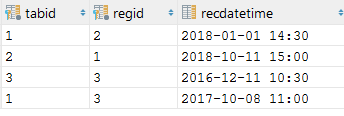
\includegraphics[scale=1]{appointment}
        \caption{Заполнение таблицы «Запись»}
        \label{fig:appointment}
\end{figure}

\vspace{0.00mm}

\cleardoublepage
\begin{figure}[!h]
        \center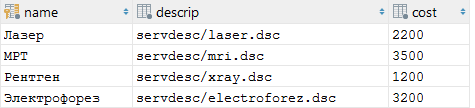
\includegraphics[scale=1]{service}
        \caption{Заполнение таблицы «Услуга»}
        \label{fig:service}
\end{figure}

\vspace{0.00mm}

\begin{figure}[h!]
        \center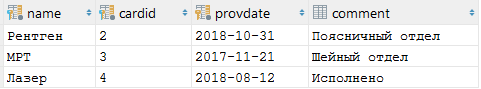
\includegraphics[scale=1]{serviceprovision}
        \caption{Заполнение таблицы «Оказание»}
        \label{fig:serviceprovision}
\end{figure}

\vspace{0.00mm}

\begin{figure}[h!]
        \center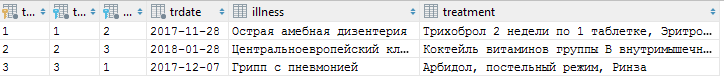
\includegraphics[scale=1]{treatment}
        \caption{Заполнение таблицы «Лечение»}
        \label{fig:treatment}
\end{figure}
\vfill
\phantom{0000}


\end{document}

